%%%%%%%%%%%%%%%%%%%%%%%%%%%%%%%%%%%%%%%%%%%%%%%%%%%%%%%%%%%%%%%%%%%%%%%%
% ICDE 2027 research paper (Round 2: submission due 11 November 2026).
% Format rules from the call for papers (https://icde2027.github.io/):
%   * IEEE conference template, PDF only.
%   * At most 12 pages, excluding references and the AI-generated content
%     acknowledgement. No appendix is allowed.
%   * Single-blind review: authors and affiliations are shown.
%   * Every author needs an ORCID at submission time.
%%%%%%%%%%%%%%%%%%%%%%%%%%%%%%%%%%%%%%%%%%%%%%%%%%%%%%%%%%%%%%%%%%%%%%%%
\documentclass[conference]{IEEEtran}
\IEEEoverridecommandlockouts

\usepackage{cite}
\usepackage{amsmath,amssymb}
\usepackage{booktabs}
\usepackage{multirow}
\usepackage{array}
\usepackage{graphicx}
\usepackage{tikz}
\usetikzlibrary{arrows.meta,positioning,fit,calc,shapes.geometric}
\usepackage{xcolor}
\usepackage{enumitem}
\usepackage{xspace}
\usepackage{algorithm}
\usepackage{algpseudocode}
\usepackage[hidelinks]{hyperref}

\definecolor{sblue}{HTML}{2B6CB0}
\definecolor{sgreen}{HTML}{2F855A}
\definecolor{sorange}{HTML}{C05621}
\definecolor{sgray}{HTML}{4A5568}
\definecolor{spurple}{HTML}{6B46C1}
\newcommand{\system}{\textsc{Synthagent}\xspace}
\newcommand{\best}[1]{\textbf{#1}}
\newcommand{\sd}[1]{\,{\tiny$\pm$#1}}
\newcommand{\resq}[1]{\textbf{RQ#1}}

% Figures are produced by generate_paper_assets.py from the ablation run.
% If a figure has not been generated yet, a framed placeholder keeps the
% manuscript compilable instead of failing the build.
\newcommand{\assetfigure}[2]{%
  \IfFileExists{#2}{\includegraphics[width=#1]{#2}}{%
    \fbox{\parbox[c][3cm][c]{\dimexpr#1-2\fboxsep-2\fboxrule\relax}{\centering\small\ttfamily missing asset: \detokenize{#2}\\ run generate\_paper\_assets.py}}}}

\begin{document}

\title{\system: A System for Reliable LLM-Based\\Synthetic Data Generation in Small Data}

% ORCIDs are entered in the submission system.
\author{%
\IEEEauthorblockN{Sancho Amaral Sim\~oes\textsuperscript{1,*},
Jo\~ao P. Vilela\textsuperscript{1,2},
Pedro Henriques Abreu\textsuperscript{1}}
\IEEEauthorblockA{\textsuperscript{1}\textit{CISUC-DEI - FCTUC, University of Coimbra}, Coimbra, Portugal\\
\textsuperscript{2}\textit{CRACS/INESCTEC-DCS - FCUP, University of Porto}, Porto, Portugal\\
\textsuperscript{*}Corresponding author\\
{\small\texttt{sanchosimoes@student.dei.uc.pt}, \texttt{jvilela@fc.up.pt}, \texttt{pha@dei.uc.pt}}}
}

\maketitle

\begin{abstract}
A dataset is small for a learning task when it holds fewer effective samples than the task requires, a common situation in healthcare. Synthetic data generation (SDG) can enlarge such datasets, but a generator fitted only to the scarce samples, such as SMOTE, a generative adversarial network or a variational autoencoder, cannot add information that those samples lack. Large language models (LLMs) can: they are not trained on the target data and generate new samples from a few real examples and the knowledge acquired during pre-training. Their output, however, is unreliable: a response can contain fewer samples than requested, malformed records, missing or invented features, or values of the wrong type, and its cost is rarely reported. This paper presents \system, a system that places a control layer between the LLM and the generated dataset. The control layer selects the real examples shown to the model, validates every response against the dataset schema, corrects invalid records, requests missing samples until the requested size is reached, and records the cost of each step. We evaluate \system on six public medical classification datasets with 195 to 768 samples and compare it with SMOTE, CTGAN and TVAE. Without any training on the target data, \system completes every run with 99.7\% to 100\% of the requested values filled. With GPT-4.1 as the LLM, it obtains the largest average F1 gain of the five generators and never lowers the average F1 of a dataset by more than 0.6 points, whereas SMOTE and CTGAN lose up to 8.2 and 10.6 points on individual datasets.
\end{abstract}

\begin{IEEEkeywords}
small data, synthetic data generation, tabular data, large language models, data augmentation, healthcare
\end{IEEEkeywords}

%======================================================================
\section{Introduction}
\label{sec:intro}
%======================================================================
\paragraph*{Context: small data}
Supervised learning assumes that the training data contain enough information to estimate a model for the target population. In healthcare this assumption often fails: a dataset is limited by the number of patients a hospital can recruit, by the prevalence of the disease, and by privacy rules that prevent pooling data across institutions~\cite{simoes2026smalldata}. Whether a dataset is too small, however, depends on the task: 300 patients can be enough to predict a common outcome from a few features and far too few for a rare outcome or many features. We therefore use the task-relative definition of our recent survey~\cite{simoes2026smalldata}, which combines learning-theoretic sample complexity with the sample-size criteria used for clinical prediction models~\cite{riley2019binary}.

\smallskip\noindent\fbox{\parbox{\dimexpr\columnwidth-2\fboxsep-2\fboxrule\relax}{%
\textbf{Definition 1 (Small data~\cite{simoes2026smalldata}).} Let $n^{\star}_{T}$ be the \emph{sample complexity} of a task $T$, the smallest number of independent, correctly labelled samples with which a model reaches a required error with high probability. Let $n_{\mathrm{eff}}(D)$ be the \emph{effective sample size} of a dataset $D$, the number of such samples that would carry the same information as $D$ once clustering, missing labels, label noise and population shift are accounted for. The \emph{smallness index} is $\sigma_T(D)=n^{\star}_{T}/n_{\mathrm{eff}}(D)$, and $D$ is \emph{small} for $T$ when $\sigma_T(D)>1$. The regimes $1<\sigma\le10$, $10<\sigma\le100$ and $\sigma>100$ are called \emph{strained}, \emph{small} and \emph{extreme}.}}\smallskip

Small data is therefore a property of the whole dataset relative to the task, not of one class. Class imbalance enters the definition only through $n^{\star}_{T}$, which for a binary outcome is driven by the number of events rather than the number of patients~\cite{riley2019binary}. The six medical datasets in our study have 195 to 768 samples; estimated with the criterion of Riley et al., their smallness index ranges from 1.0 (diabetes, at the boundary) to 42.1 (five-class heart disease), so all are small in the sense of Definition~1 (Table~\ref{tab:datasets}).

\paragraph*{Strategies for small data}
Our survey classifies remedies for small data by where the missing information comes from~\cite{simoes2026smalldata}: data from other institutions (pooling), related tasks or pre-trained models (proxy), domain knowledge (prior), unlabelled data, new data collection, and the transformation of existing data, which includes synthetic data generation (SDG). For SDG it proves a conservation result (Proposition~4.1 in~\cite{simoes2026smalldata}): a synthetic dataset produced from $D$ with the help of an external resource $M$ carries no more information about the target than $D$ and $M$ together. A generator fitted only to $D$, such as SMOTE, CTGAN or TVAE, has no $M$; it can still help a learner use $D$ more efficiently, or provide data for software testing, but it cannot add knowledge that $D$ lacks. A pre-trained generator is different: it brings the knowledge acquired on other data. This is the reason to use large language models (LLMs) for SDG in small data. An LLM is not trained on $D$; it receives a few real samples in the prompt and generates new ones using what it learned during pre-training, for example that a feature named \texttt{age} is a positive integer that increases with blood pressure~\cite{borisov2023great,seedat2024cllm}.

\paragraph*{Problem}
The difficulty is that LLM output is not reliable. A response may contain fewer samples than requested, malformed JSON, missing or invented features, or values of the wrong type (Figure~\ref{fig:teaser}, left), and every request has a cost in tokens and time. Without a mechanism that detects and corrects these failures, the output of an LLM cannot be used as a dataset. Generators fitted to $D$ have the opposite profile: their output always has the declared features and size, but in small data they estimate the distribution from the same few samples; in our experiments, only 29.6\% of the samples produced by CTGAN respect the value ranges and types of the real data (Section~\ref{sec:rq4}).

\begin{figure}[t]
\centering
\resizebox{\columnwidth}{!}{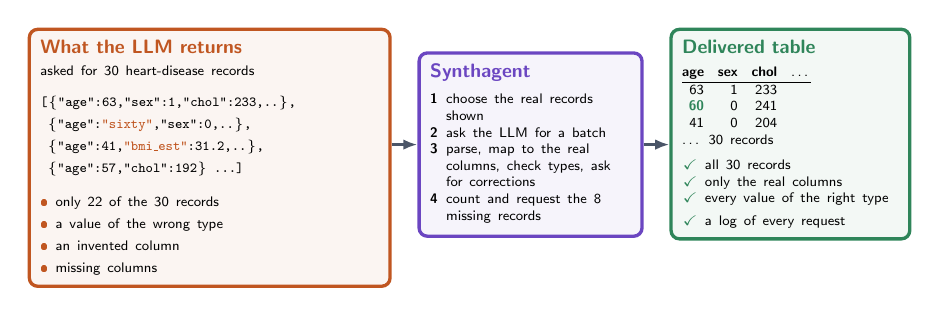
\begin{tikzpicture}[
  font=\sffamily\scriptsize,
  >={Latex[length=1.8mm]},
  box/.style={rounded corners=3pt,draw=#1,very thick,fill=#1!6,inner sep=4pt,align=left},
]
\providecommand{\bad}[1]{\textcolor{sorange}{\textbf{#1}}}
% ---------------- LLM response ----------------
\node[box=sorange,anchor=north west,text width=4.3cm] (raw) at (0,0) {%
  \textbf{\textcolor{sorange}{What the LLM returns}}\\
  {\tiny asked for 30 heart-disease records}\\[3pt]
  \texttt{\tiny [\{"age":63,"sex":1,"chol":233,..\},}\\
  \texttt{\tiny \ \{"age":\bad{"sixty"},"sex":0,..\},}\\
  \texttt{\tiny \ \{"age":41,\bad{"bmi\_est"}:31.2,..\},}\\
  \texttt{\tiny \ \{"age":57,"chol":192\} ...]}\\[4pt]
  {\tiny\bad{\textbullet} only 22 of the 30 records}\\
  {\tiny\bad{\textbullet} a value of the wrong type}\\
  {\tiny\bad{\textbullet} an invented column}\\
  {\tiny\bad{\textbullet} missing columns}};

% ---------------- Synthagent ----------------
\node[box=spurple,anchor=north west,text width=2.55cm] (ctl) at (4.95,-0.3) {%
  \textbf{\textcolor{spurple}{\system}}\\[3pt]
  {\tiny\setlength{\tabcolsep}{0pt}%
   \begin{tabular}{@{}l@{\hspace{3pt}}p{2.3cm}@{}}
   \textbf{1} & choose the real records shown\\
   \textbf{2} & ask the LLM for a batch\\
   \textbf{3} & parse, map to the real columns, check types, ask for corrections\\
   \textbf{4} & count and request the 8 missing records\\
   \end{tabular}}};

% ---------------- delivered table ----------------
\node[box=sgreen,anchor=north west,text width=2.75cm] (ok) at (8.15,0) {%
  \textbf{\textcolor{sgreen}{Delivered table}}\\[3pt]
  {\tiny\setlength{\tabcolsep}{2.5pt}%
   \begin{tabular}{@{}rrrc@{}}
   \textbf{age} & \textbf{sex} & \textbf{chol} & \dots\\\hline
   63 & 1 & 233 & \\
   \textcolor{sgreen}{\textbf{60}} & 0 & 241 & \\
   41 & 0 & 204 & \\
   \multicolumn{4}{@{}l}{\dots\ 30 records}\\
   \end{tabular}}\\[3pt]
  {\tiny\textcolor{sgreen}{\checkmark} all 30 records\\
   \textcolor{sgreen}{\checkmark} only the real columns\\
   \textcolor{sgreen}{\checkmark} every value of the right type\\
   \textcolor{sgreen}{\checkmark} a log of every request}};

\draw[->,very thick,sgray] (raw.east |- ctl.west) -- (ctl.west);
\draw[->,very thick,sgray] (ctl.east) -- (ok.west |- ctl.east);
\end{tikzpicture}
}
\caption{The problem addressed in this paper. Asked for 30 samples of a heart-disease dataset, an LLM response (left) can contain too few samples, invented or missing features and values of the wrong type. \system (right) validates and corrects every response, so the resulting dataset has the requested size and schema, and a log records each correction and its cost.}
\label{fig:teaser}
\end{figure}

\noindent\textbf{Problem statement.} \emph{Given a small dataset $D$ (Definition~1) with schema $S$ and a requested number of synthetic samples $N$, generate a synthetic dataset $G$ such that (R1) $G$ has exactly $N$ samples, (R2) every sample conforms to $S$, and (R3) the cost of generation is measured, without training a generator on $D$; and such that $G$ is (R4) faithful to $D$, (R5) does not reproduce the samples of $D$, and (R6) improves, or at least does not degrade, classifiers trained on $D$.} Requirements R1--R3 are properties a system can guarantee by construction; R4--R6 can only be measured.

\paragraph*{Existing approaches and their limitations}
Table~\ref{tab:positioning} groups existing generators by the requirements they meet. Interpolation methods such as SMOTE~\cite{chawla2002smote} need no training, but they only create samples between existing minority-class samples, add no external information and do not respect feature types. Deep generators~\cite{xu2019ctgan,kotelnikov2023tabddpm,zhang2024tabsyn} must be trained on $D$, which small data does not support, and language models fine-tuned on $D$~\cite{borisov2023great,solatorio2023realtabformer} bring pre-trained knowledge but still require training on the scarce samples. Prompted LLMs~\cite{seedat2024cllm,kim2024epic} need no training and have been proposed for the low-data setting, but they study what to include in the prompt and which generated samples to keep; they do not guarantee R1--R3. Finally, generators are usually compared from single runs. In small data this is not enough: two runs of the same generator can differ as much as two different generators (Section~\ref{sec:rq1}).

\begin{table}[t]
\centering
\caption{Requirements met by existing generator families and by \system. \checkmark: by design; (\checkmark): partially (SMOTE's size follows the class balance; fine-tuned LMs discard unparsable samples); $\times$: not addressed.}
\label{tab:positioning}
\footnotesize
\setlength{\tabcolsep}{2.5pt}
\begin{tabular*}{\columnwidth}{@{\extracolsep{\fill}}lcccc@{}}
\toprule
Family & \begin{tabular}[c]{@{}c@{}}No training\\on $D$\end{tabular} & \begin{tabular}[c]{@{}c@{}}R1: exact\\size\end{tabular} & \begin{tabular}[c]{@{}c@{}}R2: schema\\validated\end{tabular} & \begin{tabular}[c]{@{}c@{}}R3: cost\\measured\end{tabular} \\
\midrule
Interpolation~\cite{chawla2002smote} & \checkmark & (\checkmark) & $\times$ & $\times$ \\
Deep generators~\cite{xu2019ctgan,kotelnikov2023tabddpm,zhang2024tabsyn} & $\times$ & \checkmark & $\times$ & $\times$ \\
Fine-tuned LMs~\cite{borisov2023great,solatorio2023realtabformer} & $\times$ & \checkmark & (\checkmark) & $\times$ \\
Prompted LLMs~\cite{seedat2024cllm,kim2024epic} & \checkmark & $\times$ & $\times$ & $\times$ \\
\midrule
\system (ours) & \checkmark & \checkmark & \checkmark & \checkmark \\
\bottomrule
\end{tabular*}
\end{table}

\paragraph*{Our approach}
We propose \system, a system that separates two tasks: the LLM \emph{proposes} samples, and a deterministic \emph{control layer} decides which of them enter the synthetic dataset. The control layer is the part of the system that surrounds every LLM request. It keeps a record of the schema, the real samples shown to the model, the samples accepted so far and the number still missing, and it has four components, each of which removes one of the failures in Figure~\ref{fig:teaser}. A \emph{context selector} chooses which real samples fit in the prompt. A \emph{parser} repairs malformed output and maps the returned features to the schema. A \emph{validator} checks feature types and asks the model to correct only the invalid values. A \emph{completion loop} requests exactly the missing samples until $N$ is reached. Every token, correction and violation is logged. With these components, \system meets R1--R3 without training on $D$, and the experiments measure R4--R6.

\paragraph*{Research questions}
The objective of this paper is to determine whether a control layer makes LLM-based SDG a reliable and useful option for small data. We answer it through four research questions, each building on the previous one:
\begin{itemize}[leftmargin=2.8em,labelsep=.5em,itemsep=1pt]
  \item[\resq{1}] \emph{Reliability.} Does \system deliver datasets that meet R1--R3, and which components of the control layer change the result beyond the variation between repeated runs?
  \item[\resq{2}] \emph{Quality.} Are the generated samples faithful to the real data (R4) without reproducing them (R5)?
  \item[\resq{3}] \emph{Utility.} Do the generated samples improve classifiers trained on small data (R6), given how much those classifiers already vary between data splits?
  \item[\resq{4}] \emph{Comparison.} How does \system compare with established generators in quality, utility and cost, and how much does the result depend on the LLM?
\end{itemize}

\paragraph*{Contributions}
\begin{enumerate}[leftmargin=*,itemsep=1pt]
  \item \system, an open-source system that makes LLM-based SDG for small data meet R1--R3 by construction (Section~\ref{sec:system}).
  \item An evaluation protocol for SDG in small data that pairs each classifier trained with synthetic samples with the same classifier trained on real samples only, on the same data split, and that estimates the variation between repeated runs before comparing configurations (Section~\ref{sec:setup}).
  \item An empirical study on six medical datasets with four LLMs and three established generators, 780 dataset--configuration runs and up to 23,400 classifier fits (Section~\ref{sec:results}).
\end{enumerate}

\paragraph*{Main findings}
The study supports three claims. First, the control layer is sufficient to make LLM output usable as a dataset: with each of the four LLMs analysed, \system completed all six datasets and ten runs with 99.7\% to 100\% of the values filled, and the type violations of the fastest LLM were detected and sent back for correction instead of entering the dataset (RQ1). Second, with \system, LLM-based SDG is the most robust augmentation in F1 among the five generators: with GPT-4.1 it gives the largest average F1 gain ($+1.09$ points) and never lowers the average F1 of a dataset by more than 0.6 points, while SMOTE, CTGAN and TVAE lose up to 8.2, 10.6 and 2.9 points (RQ3, RQ4). Third, in small data the variation between repeated runs is as large as the effect of most design choices; only the choice of LLM exceeds it, and no generator improves utility significantly on all six datasets (RQ1, RQ4).

%======================================================================
\section{Background and Related Work}
\label{sec:related}
%======================================================================
\subsection{Synthetic Data Generation for Tabular Data}
Tabular SDG methods fall into four families. \emph{Interpolation and statistical models} include SMOTE, which creates minority-class samples on the segment between two neighbours~\cite{chawla2002smote}, and Bayesian networks, also used for differentially private release~\cite{zhang2014privbayes}. \emph{Deep generative models} learn the joint distribution with a neural network: CTGAN and TVAE~\cite{xu2019ctgan}, diffusion models such as TabDDPM, CoDi and TabSyn~\cite{kotelnikov2023tabddpm,lee2023codi,zhang2024tabsyn}, and relational or cross-silo variants~\cite{fan2020relational,shankar2024silofuse}. \emph{Fine-tuned language models} serialize each sample as text and fine-tune a language model on the target dataset: GReaT~\cite{borisov2023great}, REaLTabFormer~\cite{solatorio2023realtabformer} and TabLoft~\cite{chen2026tabloft}. \emph{Prompted LLMs} generate samples from examples placed in the prompt, without training: CLLM~\cite{seedat2024cllm} and EPIC~\cite{kim2024epic}.

\subsection{Synthetic Data Generation in Small Data}
For small data, the four families have the following limitations.
\begin{itemize}[leftmargin=*,itemsep=1pt]
  \item[L1] \emph{No external information.} Interpolation and deep generators are fitted only to $D$, so by the conservation result of~\cite{simoes2026smalldata} they cannot add information about the target; they also ignore what the features mean.
  \item[L2] \emph{Training on scarce samples.} Deep generators and fine-tuned language models estimate many parameters from the few samples available, so they can produce samples outside the observed ranges and types, or reproduce training samples~\cite{hyeong2022tabularmia}.
  \item[L3] \emph{Unreliable output.} Prompted LLMs need no training and use feature semantics, but nothing ensures that their output is a valid dataset of the requested size, and their cost is not measured. CLLM~\cite{seedat2024cllm} filters generated samples by their learning dynamics and EPIC~\cite{kim2024epic} designs balanced prompts; both focus on the quality of the samples that are kept, not on R1--R3.
  \item[L4] \emph{Evaluation without a noise estimate.} Generators are compared from single runs, so differences caused by run-to-run variation, which is large in small data, are reported as effects.
\end{itemize}
\system addresses L3 with its control layer and L4 with its evaluation protocol. Because it uses a pre-trained LLM, it also avoids L1 and L2.

\subsection{Validated Output and Data Quality}
Data-management systems have long combined generation or cleaning with integrity constraints. Kamino enforces denial constraints during private synthesis~\cite{ge2021kamino}, and data-cleaning systems combine statistical inference with constraints~\cite{chu2013holistic,qin2024bclean}. Foundation models can clean and integrate data through prompting~\cite{narayan2022wrangle}, and recovering structured records from free-form LLM output is a data-engineering problem in its own right~\cite{rorseth2026recovering}. \system applies the same principle to SDG: the schema and type rules are inferred from the data, and every LLM response is parsed and validated against them. Studies of data preparation show that a step that looks beneficial can harm downstream models~\cite{li2021cleanml,guha2023cleaningfairness}; we therefore evaluate synthetic samples with paired downstream models.

\subsection{Evaluating Synthetic Data}
Synthcity and SynthEval recommend evaluating fidelity, privacy and utility together~\cite{qian2023synthcity,lautrup2025syntheval}. A classifier two-sample test measures whether a classifier can distinguish real from synthetic samples~\cite{lopezpaz2017c2st}. Membership-inference attacks measure whether an attacker can tell which samples were used for generation~\cite{shokri2017mia,hyeong2022tabularmia}. Formal guarantees require differential privacy~\cite{dwork2014dp}, which \system does not provide; we use a membership-inference attack as a diagnostic only.

%======================================================================
\section{Problem Formulation}
\label{sec:problem}
%======================================================================
We now formalize the problem statement of Section~\ref{sec:intro}. Let $D^{\mathrm{tr}}$ and $D^{\mathrm{te}}$ be a training and a test partition of a small dataset $D$ with schema $S$. A configuration $\theta$ of the system (LLM, context strategy, active rules) produces a synthetic dataset $G_\theta$ from $D^{\mathrm{tr}}$ without access to $D^{\mathrm{te}}$. Requirements R1 and R2 define the feasible set $\mathcal{F}(S,R,N)$ of datasets with exactly $N$ samples that conform to $S$ and to the active rules $R$. The remaining requirements are objectives: a fidelity loss $L_{\mathrm{fid}}(D^{\mathrm{tr}},G_\theta)$ for R4, a privacy risk $L_{\mathrm{priv}}(D^{\mathrm{tr}},G_\theta)$ for R5, the change in downstream utility $\Delta U(G_\theta)$ for R6 and the generation cost $\kappa(\theta)$ for R3:
\begin{equation}
\theta^{\star}\in\operatorname*{arg\,min}_{\theta:\,G_{\theta}\in\mathcal{F}(S,R,N)}
\bigl(L_{\mathrm{fid}},\;L_{\mathrm{priv}},\;-\Delta U,\;\kappa\bigr)(\theta).
\label{eq:multiobjective}
\end{equation}
Equation~\eqref{eq:multiobjective} has several objectives because the requirements of Section~\ref{sec:intro} can conflict: samples that are closer to the real ones are more faithful but easier to attack, and a larger LLM may give better samples at a higher cost. We do not combine the objectives into one weighted score, because the right weights depend on the use: a hospital sharing data for software testing weights privacy and validity, while a team augmenting a classifier weights utility. \system guarantees the constraint $G_\theta\in\mathcal{F}(S,R,N)$ (Section~\ref{sec:system}); Section~\ref{sec:setup} defines how each objective is measured.

%======================================================================
\section{The \system System}
\label{sec:system}
%======================================================================
This section describes how the control layer guarantees R1--R3. Figure~\ref{fig:architecture} shows the architecture. A profiling step infers the schema $S$ and the type rules $R$ from the training data. Each generation request then goes through four stages: the context selector builds the prompt (1), the LLM proposes a batch of samples (2), the parser and validator check it (3), and the accepted samples are counted against the requested size (4). Each type of failure triggers its own correction.

\begin{figure*}[t]
\centering
\resizebox{\textwidth}{!}{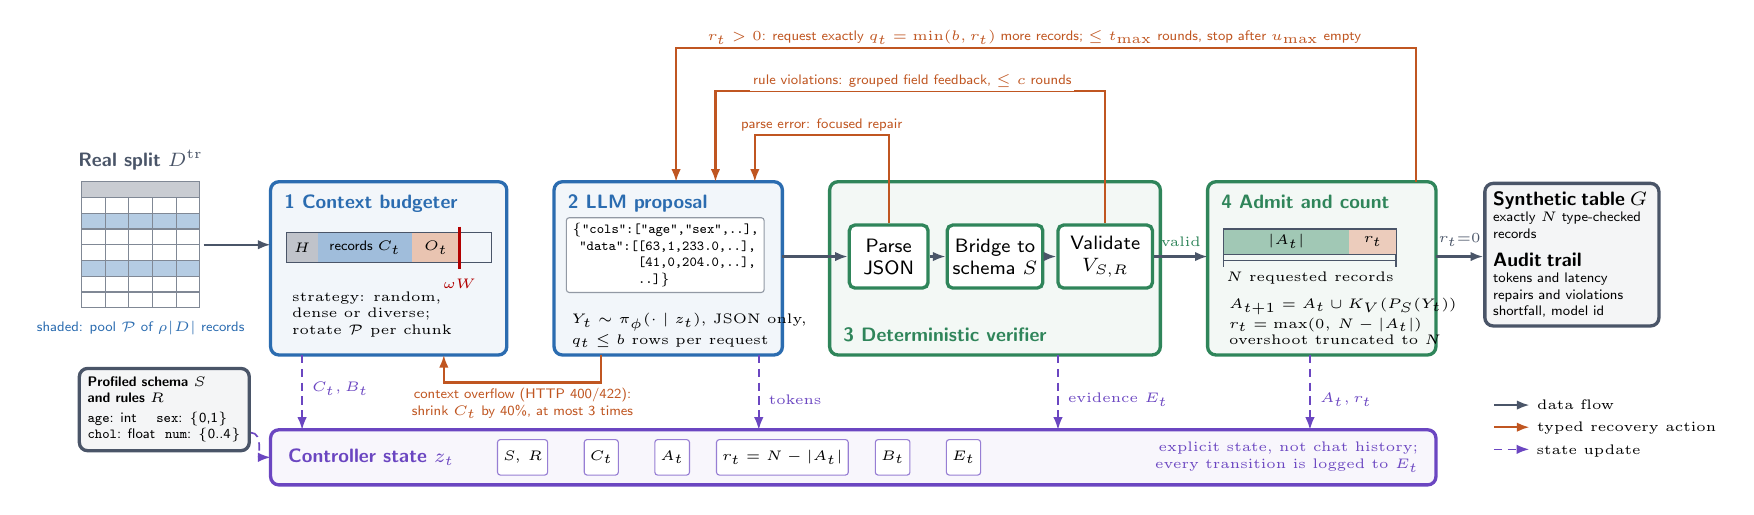
\begin{tikzpicture}[
  font=\sffamily\scriptsize,
  >={Latex[length=1.6mm]},
  flow/.style={->,thick,sgray},
  fail/.style={->,thick,sorange},
  st/.style={->,densely dashed,spurple,semithick},
  pan/.style={rounded corners=3pt,draw=#1,very thick,fill=#1!6},
  ttl/.style={font=\sffamily\bfseries\scriptsize,text=#1,anchor=north west},
  gate/.style={draw=sgreen,very thick,fill=white,rounded corners=2pt,minimum height=8mm,align=center,inner sep=2pt},
  lab/.style={font=\sffamily\tiny,text=#1,fill=white,inner sep=1pt},
]
%======================== panels ========================
\draw[pan=sblue]   (2.4,0) rectangle (5.4,-2.2);   \node[ttl=sblue]  at (2.45,-0.05) {1\,\,Context budgeter};
\draw[pan=sblue]   (6.0,0) rectangle (8.9,-2.2);   \node[ttl=sblue]  at (6.05,-0.05) {2\,\,LLM proposal};
\draw[pan=sgreen]  (9.5,0) rectangle (13.7,-2.2);  \node[ttl=sgreen,anchor=south west] at (9.55,-2.15) {3\,\,Deterministic verifier};
\draw[pan=sgreen]  (14.3,0) rectangle (17.2,-2.2); \node[ttl=sgreen] at (14.35,-0.05) {4\,\,Admit and count};

%======================== real data =====================
\foreach \r in {1,...,7}{\foreach \c in {0,...,4}{
   \ifnum\r=2 \fill[sblue!35] (\c*0.3,-\r*0.2) rectangle ++(0.3,-0.2);\fi
   \ifnum\r=5 \fill[sblue!35] (\c*0.3,-\r*0.2) rectangle ++(0.3,-0.2);\fi
   \draw[sgray!70] (\c*0.3,-\r*0.2) rectangle ++(0.3,-0.2);}}
\fill[sgray!30] (0,0) rectangle (1.5,-0.2); \draw[sgray!70] (0,0) rectangle (1.5,-0.2);
\node[font=\sffamily\bfseries\scriptsize,text=sgray,anchor=south] at (0.75,0.02) {Real split $D^{\mathrm{tr}}$};
\node[font=\sffamily\tiny,text=sblue,align=center,anchor=north] at (0.75,-1.65) {shaded: pool $\mathcal{P}$ of $\rho|D|$ records};
\draw[flow] (1.55,-0.8) -- (2.4,-0.8);

% profile card
\node[pan=sgray,anchor=north west,align=left,inner sep=3pt,font=\sffamily\tiny] (prof) at (-0.05,-2.35)
  {\textbf{Profiled schema $S$}\\\textbf{and rules $R$}\\[1pt]
   \texttt{age}: int \quad \texttt{sex}: \{0,1\}\\ \texttt{chol}: float \ \texttt{num}: \{0..4\}};

%======================== 1 budgeter ====================
\begin{scope}[shift={(2.6,-0.65)}]
  \fill[sgray!35]   (0,0) rectangle (0.4,-0.38);  \node at (0.2,-0.19)  {\tiny $H$};
  \fill[sblue!45]   (0.4,0) rectangle (1.6,-0.38); \node at (1.0,-0.19) {\tiny records $C_t$};
  \fill[sorange!35] (1.6,0) rectangle (2.2,-0.38); \node at (1.9,-0.19) {\tiny $O_t$};
  \draw[sgray] (0,0) rectangle (2.6,-0.38);
  \draw[red!70!black,thick] (2.2,0.08) -- (2.2,-0.46);
  \node[font=\tiny,text=red!70!black,anchor=north] at (2.2,-0.46) {$\omega W$};
  \node[font=\tiny,anchor=north west,align=left] at (-0.05,-0.62)
     {strategy: random,\\dense or diverse;\\rotate $\mathcal{P}$ per chunk};
\end{scope}

%======================== 2 LLM =========================
\node[anchor=north west,draw=sgray!60,fill=white,rounded corners=1pt,align=left,font=\ttfamily\tiny,inner sep=2pt]
  at (6.15,-0.45)
  {\{"cols":["age","sex",..],\\ \ "data":[[63,1,233.0,..],\\ \hphantom{\ "data":[}[41,0,204.0,..],\\ \hphantom{\ "data":[}..]\}};
\node[font=\tiny,anchor=north west,align=left] at (6.1,-1.55) {$Y_t\sim\pi_\phi(\cdot\mid z_t)$, JSON only,\\ $q_t\le b$ rows per request};

%======================== 3 verifier ====================
\node[gate,minimum width=10mm] (g1) at (10.25,-0.95) {Parse\\JSON};
\node[gate,minimum width=12mm] (g2) at (11.6,-0.95)  {Bridge to\\schema $S$};
\node[gate,minimum width=12mm] (g3) at (13.0,-0.95)  {Validate\\$V_{S,R}$};
\draw[flow] (g1)--(g2); \draw[flow] (g2)--(g3);
\draw[flow] (8.9,-0.95) -- (g1.west);

%======================== 4 admit =======================
\begin{scope}[shift={(14.5,-0.6)}]
  \fill[sgreen!45]  (0,0) rectangle (1.6,-0.32);
  \fill[sorange!30] (1.6,0) rectangle (2.2,-0.32);
  \draw[sgray] (0,0) rectangle (2.2,-0.32);
  \node at (0.8,-0.16) {\tiny $|A_t|$}; \node at (1.9,-0.16) {\tiny $r_t$};
  \draw[sgray,|-|] (0,-0.4) -- (2.2,-0.4);
  \node[font=\tiny,anchor=north] at (1.1,-0.42) {$N$ requested records};
  \node[font=\tiny,anchor=north west,align=left] at (-0.05,-0.75)
    {$A_{t+1}=A_t\cup K_V(P_S(Y_t))$\\$r_t=\max(0,\,N-|A_t|)$\\overshoot truncated to $N$};
\end{scope}
\draw[flow] (g3.east) -- node[above,font=\tiny,text=sgreen]{valid} (14.3,-0.95);

%======================== output ========================
\node[pan=sgray,anchor=north west,align=left,inner sep=3pt,text width=20mm,font=\sffamily\tiny] (out) at (17.8,0)
  {\textbf{\scriptsize Synthetic table $G$}\\exactly $N$ type-checked records\\[4pt]\textbf{\scriptsize Audit trail}\\tokens and latency\\repairs and violations\\shortfall, model id};
\draw[flow] (17.2,-0.95) -- node[above,font=\tiny]{$r_t{=}0$} (out.west|-0,-0.95);

%======================== recovery loops ================
% parse error -> focused repair
\draw[fail] (g1.north) -- (10.25,0.6) -- (8.55,0.6) -- (8.55,0);
\node[lab=sorange,anchor=south] at (9.4,0.6) {parse error: focused repair};
% violations -> grouped feedback
\draw[fail] (g3.north) -- (13.0,1.15) -- (8.05,1.15) -- (8.05,0);
\node[lab=sorange,anchor=south] at (10.55,1.15) {rule violations: grouped field feedback, $\le c$ rounds};
% residual -> top-up
\draw[fail] (16.95,0) -- (16.95,1.7) -- (7.55,1.7) -- (7.55,0);
\node[lab=sorange,anchor=south] at (12.1,1.7) {$r_t>0$: request exactly $q_t=\min(b,r_t)$ more records; $\le t_{\max}$ rounds, stop after $u_{\max}$ empty};
% overflow -> shrink context (below)
\draw[fail] (6.6,-2.2) -- (6.6,-2.55) -- (4.6,-2.55) -- (4.6,-2.2);
\node[lab=sorange,anchor=north,align=center] at (5.6,-2.58) {context overflow (HTTP 400/422):\\shrink $C_t$ by 40\%, at most 3 times};

%======================== state register ================
\draw[draw=spurple,very thick,fill=spurple!5,rounded corners=3pt] (2.4,-3.15) rectangle (17.2,-3.85);
\node[font=\sffamily\bfseries\scriptsize,text=spurple,anchor=west] at (2.5,-3.5) {Controller state $z_t$};
\foreach \lab/\x in {{$S,\,R$}/5.6,{$C_t$}/6.6,{$A_t$}/7.5,{$r_t=N-|A_t|$}/8.9,{$B_t$}/10.3,{$E_t$}/11.2}{
  \node[draw=spurple!70,fill=white,rounded corners=1pt,minimum height=4.5mm,inner sep=2pt,font=\tiny] at (\x,-3.5) {\lab};}
\node[font=\tiny,text=spurple,anchor=east,align=right] at (17.1,-3.5) {explicit state, not chat history;\\every transition is logged to $E_t$};
\draw[st] (prof.south east) ++(0,0.25) to[out=0,in=180] (2.4,-3.5);
\draw[st] (2.8,-2.2) -- (2.8,-3.15) node[pos=.45,right,font=\tiny]{$C_t,B_t$};
\draw[st] (8.6,-2.2) -- (8.6,-3.15) node[pos=.6,right,font=\tiny]{tokens};
\draw[st] (12.4,-2.2) -- (12.4,-3.15) node[pos=.6,right,font=\tiny]{evidence $E_t$};
\draw[st] (15.6,-2.2) -- (15.6,-3.15) node[pos=.6,right,font=\tiny]{$A_t,r_t$};

%======================== legend ========================
\node[anchor=north west,font=\tiny,align=left] at (17.8,-2.65) {
  \tikz\draw[flow](0,0)--(0.45,0); data flow\\[2pt]
  \tikz\draw[fail](0,0)--(0.45,0); typed recovery action\\[2pt]
  \tikz\draw[st](0,0)--(0.45,0); state update};
\end{tikzpicture}
}
\caption{Architecture of \system. Real samples enter a context window of limited size (1); the LLM proposes a JSON batch (2); deterministic checks parse it, map it to the schema and validate the type rules (3); and accepted samples are counted against the requested size (4). Each failure type triggers its own correction (orange). Every stage reads or updates the state $z_t$ of the control layer (purple), which also serves as the audit log of the run.}
\label{fig:architecture}
\end{figure*}

\subsection{State of the Control Layer}
Let $D^{\mathrm{tr}}$ be the training data with schema $S$, $N$ the requested number of synthetic samples and $R$ the active rules. At step $t$, the control layer keeps the state
\begin{equation}
z_t=(S,\,R,\,C_t,\,A_t,\,N-|A_t|,\,B_t,\,E_t),
\label{eq:state}
\end{equation}
where $C_t$ is the set of real samples shown to the LLM, $A_t$ the accepted synthetic samples, $N-|A_t|$ the number still missing, $B_t$ the remaining token budget and $E_t$ the log of parser and validator results. The LLM, denoted $\pi_{\phi}$, proposes a batch $Y_t\sim\pi_{\phi}(\cdot\mid z_t)$. Let $P_S$ be the parser, which also maps the returned features to $S$, $V_{S,R}$ the validator and $K$ a correction step that sends the invalid values back to the LLM, at most twice. The accepted set is updated as
\begin{equation}
A_{t+1}=A_t\cup K_{V_{S,R}}\bigl(P_S(Y_t)\bigr).
\label{eq:acceptance}
\end{equation}
Equation~\eqref{eq:acceptance} expresses the main design decision: the LLM only proposes, and a sample enters $A_{t+1}$ only after it has been parsed, mapped to $S$ and validated. The state is explicit rather than implied by the conversation history, so the number of missing samples is always known, and $E_t$ records every failure for later inspection.

\subsection{Context Selection (R1, R3)}
The context selector decides which real samples the LLM sees. Table~\ref{tab:prompt-context} lists exactly what the model receives in our experiments. The core evidence is a 20\% sample of the real training split, serialized as compact row-major JSON with the ordered feature columns and the observed target, so the model sees how features and class co-occur in real samples. No free-text description of the clinical task is added, so that no dataset receives more prompt engineering than another; the model must infer the role of each feature from its name and values.

\begin{table*}[t]
\centering
\caption{Information boundary for one generation request in the reported study. ``Not supplied'' is intentional: those signals cannot influence the generated rows.}
\label{tab:prompt-context}
\small
\begin{tabular}{p{.17\textwidth}p{.36\textwidth}p{.39\textwidth}}
\toprule
Context layer & What the model receives & Why it is included or excluded \\
\midrule
Schema & Ordered column names and an exact column-count requirement & Fixes the record interface and prevents invented or omitted fields. \\
Demonstrations & Compact row-major serialization of a 20\% sample of the training split, with feature and target values & Exposes joint patterns, value formats, label prevalence and plausible cross-column combinations without sending the whole local table. \\
Generation task & Exact number of new rows for the current chunk, at most 30 & Turns an open-ended completion into a bounded action whose output count can be verified. \\
Output contract & JSON only, fixed column order, complete cells, raw numeric values, no extra metadata & Makes parsing deterministic and removes interface failures unrelated to statistical quality. \\
Dynamic feedback & Parser error location after malformed JSON, or grouped field violations after failed validation & Reveals only the evidence needed for a targeted repair instead of replaying the full history. \\
Free-text metadata & Not supplied & Prevents unequal, dataset-specific prompt engineering from confounding the comparison. \\
Test information & No holdout rows, predictions, metrics or classifier identities & Preserves the evaluation boundary and prevents optimization against the test set. \\
Global statistics & No separately computed means, quantiles, correlations or class quotas & Fidelity must arise from the selected rows; the consequence is weaker protection against rare-mode omission. \\
\bottomrule
\end{tabular}
\end{table*}

Formally, a selection strategy $s\in\{\text{random},\text{dense},\text{diverse}\}$ defines an ordered candidate pool, and the token budget determines how much of that pool is visible:
\begin{equation}
\begin{aligned}
C_t&=\operatorname{Slice}_{t}\!\left(\operatorname{Select}_{s}
(D^{\mathrm{tr}},\lceil0.2|D^{\mathrm{tr}}|\rceil),k_t\right),\\
k_t&=\max\{k:T(H,I,C_{t,k},O_t)\leq0.85W\}.
\end{aligned}
\label{eq:context}
\end{equation}
Here $H$ is the schema and output contract, $I$ optional instruction text, $O_t$ the reserved output, $W$ the backend context window and $T$ a token estimator (2.8 characters per token for compact JSON). The slice operator rotates through the pool across chunks, so successive requests see different patients when the pool exceeds one window. If the provider still rejects a request as too long (HTTP 400 or 422), the control layer shrinks the visible context by 40\% and retries, at most three times. ``20\% context'' therefore describes the candidate pool, not a promise that every candidate row appears in every prompt.

The 20\% fraction and the 85\% window limit were fixed before the experiments and not tuned. The default strategy samples the context at random. \emph{Dense} prefers rows with the most observed cells, reducing ambiguity from missing fields. \emph{Diverse} standardizes numerical features, runs $k$-means and selects the rows nearest to the centroids, so that the context covers more of the feature space. Neither strategy is class-stratified, so neither guarantees that a rare diagnosis appears in context; Section~\ref{sec:discussion} returns to this limitation.

\subsection{Parsing, Validation and Correction (R2)}
The parser and the validator decide which parts of a response can enter the accepted set $A_t$ of Equation~\eqref{eq:acceptance}.
Samples are requested in JSON batches of at most 30, a size that keeps every response within the output limit of the smallest LLM tested and limits the loss when a response fails. A local parser first extracts structured content and fixes common defects (non-finite literals, trailing commas, concatenated objects). If parsing still fails, the control layer issues one repair request at temperature 0.1 that quotes the error position and surrounding text. The returned feature names are then mapped back to the schema.

Profiling infers a type rule for every feature, and optional boundary rules (numerical ranges with 10\% tolerance, or categorical domains with at most 20 values). Dynamic Pydantic models validate each batch. The validator groups failures by field and reports one representative bad value per field, so the correction prompt does not grow linearly with repeated errors. Up to two correction rounds are attempted per batch. User-defined post-processing rules (noise, rounding, normalization) can be applied deterministically afterwards.

In the reference configuration of our experiments, type rules are active, boundary rules are off and no user rules are supplied, so we evaluate the default system rather than the strictest one. Rules are used only by the validator and are never inserted into the prompt.

\subsection{Completion Loop (R1)}
LLMs often return fewer samples than requested. The completion loop derives its next request from the accepted state rather than from the conversation:
\begin{equation}
r_t=\max(0,N-|A_t|),\qquad q_t=\min(30,r_t).
\label{eq:residual}
\end{equation}
Equation~\eqref{eq:residual} requests only the residual $q_t$, and any overshoot is truncated. The loop runs for at most 50 top-up rounds and stops after five consecutive empty or unparsable responses. Successful runs therefore return exactly $N$ rows; persistent provider failure can still end a run short, and that shortfall is recorded rather than hidden. Algorithm~\ref{alg:loop} summarizes the complete loop.

\begin{algorithm}[t]
\caption{Generation loop of the control layer}
\label{alg:loop}
\small
\begin{algorithmic}[1]
\Require table $D^{\mathrm{tr}}$, schema $S$, rules $R$, volume $N$, strategy $s$, window $W$
\State $\mathcal{P}\gets\operatorname{Select}_s(D^{\mathrm{tr}},\lceil0.2|D^{\mathrm{tr}}|\rceil)$; $A\gets\emptyset$; $E\gets[\,]$
\For{chunk $t=1,\dots,\lceil N/30\rceil$}
  \State $C_t\gets$ rotated slice of $\mathcal{P}$ that fits $0.85W$ \Comment{Eq.~\eqref{eq:context}}
  \State $Y\gets\pi_\phi(S,C_t,\min(30,N-30(t-1)))$; on overflow shrink $C_t$ by 40\%, retry $\le3$
  \State $X\gets P_S(Y)$; \textbf{if} parse fails \textbf{then} $X\gets P_S(\text{repair}(Y))$
  \For{$j=1,2$} \Comment{targeted correction}
    \State \textbf{if} $V_{S,R}(X)$ has no violations \textbf{then break}
    \State $X\gets P_S(\pi_\phi(\text{grouped violations of }X))$; append to $E$
  \EndFor
  \State $A\gets A\cup X$
\EndFor
\State $u\gets0$
\While{$|A|<N$ \textbf{and} fewer than 50 rounds \textbf{and} $u<5$} \Comment{Eq.~\eqref{eq:residual}}
  \State $X\gets P_S(\pi_\phi(S,\text{first 20 rows of }\mathcal{P},\min(30,N-|A|)))$
  \State \textbf{if} $X=\emptyset$ \textbf{then} $u\gets u+1$ \textbf{else} $A\gets A\cup X$; $u\gets0$
\EndWhile
\State \Return first $N$ rows of $A$, together with $E$, token counts and timings
\end{algorithmic}
\end{algorithm}

\paragraph*{Audit log and cost accounting (R3)}
Every run records prompt, completion and total tokens, LLM generation time, parser repair attempts, rule violations, the requested and delivered row counts and the model identifier. These records make a synthetic dataset inspectable after the fact and give the cost term $\kappa(\theta)$ in Equation~\eqref{eq:multiobjective} a measured value.

%======================================================================
\section{Experimental Setup}
\label{sec:setup}
%======================================================================
This section describes the data, protocol and measures used to answer RQ1--RQ4, and justifies each choice.

\subsection{Datasets}
We use healthcare data because it is the domain where small data is most common and where the motivation for SDG, more training samples without exposing patients, is strongest~\cite{simoes2026smalldata}. We use public datasets so that every result can be reproduced. Table~\ref{tab:datasets} lists the six classification datasets. Five come from the UCI repository~\cite{uciheart,ucibreast,uciheartfailure,uciilpd,uciparkinsons}, and the diabetes dataset is the Pima Indians benchmark~\cite{smith1988diabetes}. They were chosen because they are widely used benchmarks, they are all small in the sense of Definition~1, and together they cover the factors that make small data harder: sample sizes from 195 to 768, 8 to 30 features, two to five classes, a smallest class from 4.3\% to 37.3\% of the samples, and smallness indices across the strained and small regimes. We keep the original five-class heart-disease target. Missing values (0.1\% of the cells in two datasets) are imputed with the mean for numerical and the mode for categorical features.

\begin{table}[t]
\centering
\caption{Evaluation datasets. $n$: samples; $d$: features; $k$: classes; $n_{\min}$: samples in the smallest class; $n^{\star}$: sample complexity by the first criterion of Riley et al.~\cite{riley2019binary} (shrinkage 0.9, $d(k-1)$ parameters, anticipated $R^2_{\mathrm{CS}}$ of 15\% of its maximum); $\sigma=n^{\star}/n_{\mathrm{eff}}$ with $n_{\mathrm{eff}}$ the training size ($0.8n$).}
\label{tab:datasets}
\footnotesize
\setlength{\tabcolsep}{3pt}
\begin{tabular*}{\columnwidth}{@{\extracolsep{\fill}}lrrrrrr@{}}
\toprule
Dataset & $n$ & $d$ & $k$ & $n_{\min}$ (\%) & $n^{\star}$ & $\sigma$ \\
\midrule
Heart disease & 303 & 13 & 5 & 13 (4.3) & 10,201 & 42.1 \\
Breast cancer & 569 & 30 & 2 & 212 (37.3) & 2,302 & 5.1 \\
Heart failure & 299 & 12 & 2 & 96 (32.1) & 946 & 4.0 \\
Diabetes & 768 & 8 & 2 & 268 (34.9) & 621 & 1.0 \\
Liver disease & 583 & 10 & 2 & 167 (28.6) & 808 & 1.7 \\
Parkinson's & 195 & 22 & 2 & 48 (24.6) & 1,851 & 11.9 \\
\bottomrule
\end{tabular*}
\par\vspace{2pt}\raggedright\scriptsize For heart disease, $n^{\star}$ applies the binary criterion to the smallest class versus the rest and is an approximation. Parkinson's contains several recordings per subject, so its true $n_{\mathrm{eff}}$ is lower and its $\sigma$ higher than shown.
\end{table}

\subsection{Protocol}
Measuring whether synthetic samples help a classifier requires real samples that the generator has never seen, so each dataset is split into a training partition, given to the generator, and a test partition, used only to score classifiers. In small data a single split is unreliable, because the test partition holds only 39 to 154 samples and the result changes with the split. We therefore repeat the split ten times with seeds 43 to 52 (80/20 holdouts) and report means and standard deviations. In each repetition, the generator receives the training partition and produces as many synthetic samples as there are training samples; the LLM sees a 20\% sample of the training partition as context. Generation uses temperature 0.3, a value chosen in advance to favour adherence to the output format while keeping some diversity.

\paragraph*{Classifiers}
The utility of synthetic data depends on the learner: interpolated samples can help a nearest-neighbour classifier and harm a boosted ensemble. To avoid conclusions tied to one learner, we train ten classifiers that cover the main model families: linear (logistic regression, LR), kernel (support vector machine, SVM), distance-based ($k$-nearest neighbours, $k$NN), probabilistic (Gaussian naive Bayes, NB), a single tree (decision tree, DT), bagging (random forest, RF), boosting (gradient boosting, GB; AdaBoost; XGBoost) and a neural network (multilayer perceptron, MLP). Each classifier is trained in three regimes on the same test partition: real samples only, synthetic samples only, and real plus synthetic samples. XGBoost failed on liver disease in every repetition because its labels are coded $\{1,2\}$; the code now re-encodes them, but filling this cell would require regenerating every configuration, so we report 59 of 60 classifier--dataset cells.

\subsection{Configurations}
We evaluate 13 configurations; only those that completed all six datasets and ten repetitions are analysed. To answer RQ1, seven \emph{control-layer variants} use GPT-4o mini: the reference \system; three variants that disable a component (type rules, post-processing, and a legacy context-join option); dense and diverse context selection; and a variant in which the LLM chooses context size, selection strategy and temperature from a profile of the dataset. To answer RQ4, four \emph{LLMs} run the reference configuration: GPT-4o mini, GPT-4.1 mini, GPT-4o and GPT-4.1. They form a $2\times2$ design that crosses model generation (4o versus 4.1) with model size (full versus mini). Using one provider keeps the interface, tokenizer and output mode constant, so differences can be attributed to the model; GPT-4o mini, the cheapest, is the reference so that every variant runs at the lowest cost. The control layer itself works with any OpenAI-compatible endpoint, including locally served open models. Three \emph{established generators} use the same splits: SMOTE~\cite{chawla2002smote}, which balances every class to the majority count and therefore emits only non-majority samples, and CTGAN and TVAE~\cite{xu2019ctgan} with the default settings of the reference implementation (300 epochs). In total, 13 configurations give 780 dataset--configuration runs and up to 23,400 classifier fits.

Three control-layer variants turn out to change nothing in this setting. With no user rules, disabling post-processing removes a step that does nothing; the context-join option affects only a legacy fidelity score; and disabling type rules cannot change the result because the reference validator never found a violation with GPT-4o mini. Together with the reference, these variants are four independent runs of the same pipeline. Their spread estimates the variation between repeated runs, which we call the \emph{noise floor}: a difference between two configurations smaller than this spread is not evidence of an effect.

\subsection{Measures}
Each requirement of Section~\ref{sec:intro} is measured as follows. \emph{R1--R3 (reliability):} completeness, the percentage of non-empty values in the synthetic dataset; the number of parser repairs and type violations; and the cost in tokens and generation time. \emph{R4 (fidelity):} computed on the synthetic samples alone, without the real context, for the numerical features $\mathcal{J}$:
\begin{equation}
\begin{aligned}
F_{\mathrm{JSD}}&=100\Bigl(1-\tfrac{1}{|\mathcal{J}|}
\textstyle\sum_{j\in\mathcal{J}}D_{\mathrm{JS}}(D_j,G_j)\Bigr),\\
F_{\mathrm{corr}}&=100\bigl(1-\operatorname{mean}|\Sigma_D-\Sigma_G|\bigr),
\end{aligned}
\label{eq:fidelity}
\end{equation}
where $D_{\mathrm{JS}}$ is the Jensen--Shannon divergence between real and synthetic marginals and $\Sigma_D$, $\Sigma_G$ are the correlation matrices; both scores are 100 for identical distributions. We also report a classifier two-sample test (C2ST)~\cite{lopezpaz2017c2st}: a random forest is trained to separate real from synthetic samples, and an accuracy close to 0.5 means they are hard to distinguish. For the established generators, we also report the percentage of \emph{valid} samples, those whose values lie in the observed ranges and categories and are integers where the real feature is. \emph{R5 (privacy):} a membership-inference attack scores each real sample by its distance to the nearest synthetic sample and reports the ROC AUC for training versus test samples; 0.5 is chance. \emph{R6 (utility):} for metric $m\in\{\mathrm{accuracy},\mathrm{F1}\}$, dataset $d$, classifier $c$ and repetition $h$,
\begin{equation}
\Delta m_{d,c,h}=m\bigl(D^{\mathrm{tr}}_{d,h}\cup G_{d,h};\,c\bigr)-m\bigl(D^{\mathrm{tr}}_{d,h};\,c\bigr),
\label{eq:utility}
\end{equation}
with both models scored on the same test partition, so that the variation between test partitions does not appear as an effect of SDG. We use binary F1 for the binary tasks and class-weighted F1 for heart disease. Binary F1 scores the class coded 1, which is the minority class for heart failure and diabetes and the majority class for liver disease and Parkinson's. Changes are reported in percentage points (pp).

\subsection{Statistical Analysis}
Repetitions and classifiers are not independent datasets, so we average them within each dataset and treat the six datasets as matched blocks. Configurations are compared with the Friedman test,
\begin{equation}
\chi^2_F=\frac{12M}{Q(Q+1)}\sum_{a=1}^{Q}\bar{\mathrm{rk}}_a^{\,2}-3M(Q+1),
\label{eq:friedman}
\end{equation}
where $\bar{\mathrm{rk}}_a$ is the average rank of configuration $a$ over $M=6$ datasets and $Q$ the number of configurations, followed by two-sided Wilcoxon signed-rank tests of the best-ranked configuration against every other, with Holm correction~\cite{demsar2006statistical,holm1979procedure}. Per-cell tests of augmented versus real-only training over the ten repetitions are Holm-corrected within each metric. With six blocks the tests have limited power, so we report effect sizes and the noise floor alongside $p$-values.

%======================================================================
\section{Results}
\label{sec:results}
%======================================================================
\subsection{RQ1: Reliability of the Control Layer}
\label{sec:rq1}
\paragraph*{R1--R3 are met} Every analysed configuration completed all six datasets and ten repetitions. The synthetic datasets have 99.7\% of their values filled with GPT-4o mini and 100.0\% with the other three LLMs. The control layer also recorded when its components were needed. With GPT-4o mini, GPT-4o and GPT-4.1, no response needed a JSON repair and no sample violated a type rule. GPT-4.1 mini, the fastest LLM, produced on average 7.4 type violations per repetition on breast cancer and one malformed response in ten repetitions on diabetes. These were detected and sent back for correction instead of entering the dataset, and the resulting datasets were complete and gave the best mean accuracy change of all configurations (Table~\ref{tab:backend}). A faster but less disciplined LLM can therefore be used, because its failures are caught. Cost is measured for every run: 72,000 to 81,000 tokens per repetition for the LLM configurations (Table~\ref{tab:ablation}).

\paragraph*{The noise floor} Table~\ref{tab:ablation} compares the control-layer variants. The first four rows are the same pipeline, so their spread is the noise floor: JSD 72.43--72.92, correlation 70.83--72.93, mean accuracy change $-1.80$ to $-1.19$ pp, mean F1 change $-0.18$ to $+0.28$ pp and attack AUC 0.523--0.534. Differences of about 0.5 JSD points, 2 correlation points or 0.6 pp of utility between two runs are therefore not evidence of a design effect. Generation time is not a reliable cost measure: the four equivalent runs take 228 to 379 seconds per repetition, depending on the provider, while their token counts differ by less than 2\%. We therefore use tokens as the cost measure.

\begin{table*}[t]
\centering
\caption{Control-layer variants (RQ1), all with GPT-4o mini. The first four rows run the same pipeline and define the noise floor. Seconds and tokens are means per repetition. Bold: best value among the LLM configurations; lower is better for C2ST, for the distance of the attack AUC from 0.5, and for cost.}
\label{tab:ablation}
\footnotesize
\begin{tabular*}{\textwidth}{@{\extracolsep{\fill}}lrrrrrrrr@{}}
\toprule
& \multicolumn{4}{c}{Fidelity (R4) and privacy (R5)} & \multicolumn{2}{c}{Utility change (R6, pp)} & \multicolumn{2}{c}{Cost per repetition (R3)} \\
\cmidrule(lr){2-5}\cmidrule(lr){6-7}\cmidrule(l){8-9}
Configuration & JSD & Corr. & C2ST & Attack AUC & Acc. & F1 & Seconds & Tokens \\
\midrule
\multicolumn{9}{l}{\textit{Noise floor: four runs of the same pipeline}}\\
Reference \system & 72.70 & 72.57 & 0.878 & 0.526 & \best{$-1.19$} & $-0.14$ & 378.7 & 73,510 \\
No type rules & 72.92 & 72.93 & 0.876 & 0.534 & $-1.80$ & $-0.04$ & 321.6 & \best{72,188} \\
No post-processing & 72.43 & 70.83 & 0.883 & \best{0.523} & $-1.71$ & \best{$+0.28$} & 251.5 & 72,235 \\
No context join & 72.52 & 71.18 & 0.880 & 0.531 & $-1.31$ & $-0.18$ & \best{228.1} & 72,576 \\
\midrule
\multicolumn{9}{l}{\textit{Design choices}}\\
Dense context & 72.87 & 70.88 & 0.878 & 0.525 & $-1.24$ & $+0.07$ & 238.8 & 72,600 \\
Diverse context & \best{73.27} & \best{73.72} & \best{0.872} & 0.544 & $-1.34$ & $-0.13$ & 271.1 & 73,757 \\
LLM-chosen settings & 72.53 & 70.10 & 0.886 & 0.526 & $-1.25$ & $+0.11$ & 310.2 & 115,245 \\
\bottomrule
\end{tabular*}
\end{table*}

\paragraph*{Effect of the design choices} Against this floor, the design choices have small effects. Dense context stays inside the floor on every measure. Diverse context is the only choice that leaves it on fidelity, with the highest JSD (73.27) and correlation (73.72) and the lowest C2ST accuracy (0.872), but also the highest attack AUC (0.544): samples that cover more of the feature space are closer to more real samples. Letting the LLM choose its own settings stays inside the floor on fidelity and utility and costs 57\% more tokens (115,245 versus 73,510). The Friedman tests find no difference in utility between the variants ($\chi^2_F(7)=3.10$, $p=.875$ for accuracy; $\chi^2_F(7)=4.39$, $p=.734$ for F1), and every Holm-adjusted comparison has $p=1.0$ (Figure~\ref{fig:ranks}).

\begin{figure}[t]
\centering
\assetfigure{\columnwidth}{generated/architecture_ranks.pdf}
\caption{Average ranks of the control-layer variants and SMOTE over the six datasets (lower is better). Neither accuracy nor F1 shows a significant difference.}
\label{fig:ranks}
\end{figure}

\noindent\textit{Answer to RQ1.} \system meets R1--R3 with every LLM analysed: the datasets are complete, failures are detected and corrected, and cost is recorded. Within one LLM, no design choice changes fidelity or utility by more than the noise floor, except a small fidelity gain from diverse context. The value of the control layer is reliability, not a higher score.

\subsection{RQ2: Fidelity and Privacy}
\label{sec:rq2}
Table~\ref{tab:full} reports the reference configuration per dataset. Marginal fidelity averages 72.7 out of 100, from 65.2 on the five-class heart-disease dataset, the smallest in the sense of Definition~1, to 80.2 on diabetes, the largest. The membership-inference attack stays near chance: 0.526 on average and at most 0.567 on any dataset, so the synthetic samples do not reveal which real samples were used. This is a diagnostic for one attack, not a formal guarantee. The C2ST accuracy of 0.878 shows that a classifier can still separate real from synthetic samples; we therefore do not claim that the synthetic samples can replace real ones.

\begin{table}[t]
\centering
\caption{Reference configuration (GPT-4o mini) per dataset, averaged over ten repetitions and all classifiers (RQ2, RQ3). JSD and correlation are on a 0--100 scale.}
\label{tab:full}
\footnotesize
\setlength{\tabcolsep}{2.2pt}
\begin{tabular*}{\columnwidth}{@{\extracolsep{\fill}}lrrrrrrrr@{}}
\toprule
& \multicolumn{4}{c}{R4 and R5} & \multicolumn{2}{c}{Acc.\ (\%)} & \multicolumn{2}{c}{Change (pp)} \\
\cmidrule(lr){2-5}\cmidrule(lr){6-7}\cmidrule(l){8-9}
Dataset & JSD & Corr. & C2ST & AUC & Real & Aug. & Acc. & F1 \\
\midrule
Breast & 77.2 & 74.5 & 0.911 & 0.550 & 95.1 & 94.4 & $-0.66$ & $-0.62$ \\
Diabetes & 80.2 & 44.0 & 0.897 & 0.504 & 74.2 & 74.1 & $-0.03$ & $+2.39$ \\
Heart dis. & 65.2 & 76.6 & 0.893 & 0.507 & 56.6 & 53.4 & $-3.15$ & $-0.97$ \\
Heart fail. & 71.2 & 81.2 & 0.892 & 0.534 & 74.1 & 71.6 & $-2.53$ & $-1.00$ \\
Liver & 71.8 & 73.8 & 0.883 & 0.495 & 67.4 & 67.6 & $+0.19$ & $+0.13$ \\
Parkinson's & 70.6 & 85.3 & 0.789 & 0.567 & 84.9 & 84.0 & $-0.97$ & $-0.77$ \\
\midrule
Mean & 72.7 & 72.6 & 0.878 & 0.526 & 75.4 & 74.2 & $-1.19$ & $-0.14$ \\
\bottomrule
\end{tabular*}
\end{table}

\noindent\textit{Answer to RQ2.} The synthetic samples follow the real marginals reasonably well, without reproducing the real samples, but they remain distinguishable from real data.

\subsection{RQ3: Utility for Classifiers Trained on Small Data}
\label{sec:rq3}
\paragraph*{Variation of the real-only baselines} Before measuring the effect of synthetic samples, we measure how much classifiers trained on real data alone vary between splits (Table~\ref{tab:baselines}). This variation is the yardstick for every utility effect. On the 195-sample Parkinson's dataset, MLP accuracy is $72.3\pm18.2\%$, while tree ensembles exceed 92\%. On heart failure, SVM and $k$NN reach 63.3\% and 61.3\% accuracy but an F1 of 0.0 and 0.7, because they almost never predict the minority class; accuracy alone would hide the failure that SDG is meant to address.

\begin{table*}[t]
\centering
\caption{Real-only baselines (RQ3) over ten 80/20 splits: mean in percent, standard deviation in small type. XGBoost on liver disease (--) failed in every split because the labels are coded $\{1,2\}$.}
\label{tab:baselines}
\footnotesize
\setlength{\tabcolsep}{2pt}
\begin{tabular*}{\textwidth}{@{\extracolsep{\fill}}lrrrrrrrrrrrr@{}}
\toprule
 & \multicolumn{2}{c}{Heart dis.} & \multicolumn{2}{c}{Breast} & \multicolumn{2}{c}{Heart fail.} & \multicolumn{2}{c}{Diabetes} & \multicolumn{2}{c}{Liver} & \multicolumn{2}{c}{Parkinson's} \\
\cmidrule(lr){2-3} \cmidrule(lr){4-5} \cmidrule(lr){6-7} \cmidrule(lr){8-9} \cmidrule(lr){10-11} \cmidrule(lr){12-13}
Classifier & Acc. & F1 & Acc. & F1 & Acc. & F1 & Acc. & F1 & Acc. & F1 & Acc. & F1 \\
\midrule
RF & 61.0\sd{4.4} & 57.0\sd{5.9} & 95.6\sd{1.8} & 95.0\sd{2.8} & 84.3\sd{3.3} & 76.8\sd{4.4} & 74.9\sd{2.8} & 60.4\sd{6.0} & 71.1\sd{3.5} & 81.4\sd{2.4} & 92.3\sd{3.2} & 94.8\sd{2.2} \\
DT & 53.4\sd{3.9} & 54.0\sd{5.0} & 93.3\sd{2.3} & 92.1\sd{4.0} & 79.2\sd{4.7} & 68.4\sd{9.2} & 71.1\sd{3.8} & 57.2\sd{6.4} & 66.0\sd{3.2} & 76.3\sd{3.1} & 85.1\sd{5.6} & 89.7\sd{3.8} \\
MLP & 56.6\sd{6.4} & 52.5\sd{7.6} & 94.7\sd{0.9} & 94.0\sd{2.1} & 48.3\sd{12.9} & 34.2\sd{24.7} & 68.4\sd{4.1} & 52.9\sd{12.0} & 68.4\sd{4.1} & 79.4\sd{3.6} & 72.3\sd{18.2} & 77.8\sd{26.1} \\
SVM & 54.8\sd{6.8} & 39.0\sd{7.9} & 93.3\sd{2.1} & 92.4\sd{3.4} & 63.3\sd{5.2} & 0.0\sd{0.0} & 75.6\sd{2.2} & 57.3\sd{4.7} & 70.7\sd{2.9} & 82.8\sd{2.0} & 81.0\sd{8.2} & 88.5\sd{5.2} \\
LR & 59.8\sd{5.6} & 56.5\sd{5.0} & 95.2\sd{2.0} & 94.6\sd{2.6} & 80.5\sd{3.6} & 68.9\sd{8.4} & 77.3\sd{2.0} & 62.8\sd{5.4} & 70.3\sd{4.0} & 81.1\sd{3.2} & 86.9\sd{5.6} & 91.3\sd{3.9} \\
kNN & 55.4\sd{6.3} & 44.4\sd{7.9} & 94.3\sd{1.8} & 93.4\sd{3.2} & 61.3\sd{4.1} & 0.7\sd{2.1} & 75.5\sd{1.8} & 60.0\sd{3.3} & 68.6\sd{4.2} & 79.7\sd{3.2} & 83.6\sd{5.6} & 89.5\sd{3.9} \\
NB & 55.7\sd{5.3} & 56.9\sd{5.0} & 93.9\sd{1.7} & 93.1\sd{3.2} & 75.0\sd{4.9} & 56.7\sd{13.1} & 76.4\sd{2.4} & 64.0\sd{4.9} & 55.9\sd{3.7} & 55.9\sd{3.8} & 71.5\sd{4.4} & 76.6\sd{4.0} \\
GB & 54.1\sd{5.5} & 52.8\sd{6.3} & 95.9\sd{2.2} & 95.4\sd{2.8} & 83.0\sd{4.9} & 75.4\sd{7.2} & 74.7\sd{3.0} & 61.7\sd{5.8} & 67.9\sd{3.3} & 78.7\sd{2.4} & 92.1\sd{4.0} & 94.7\sd{2.6} \\
AdaBoost & 60.8\sd{7.6} & 60.7\sd{7.3} & 97.1\sd{1.5} & 96.8\sd{1.7} & 82.5\sd{3.0} & 74.2\sd{6.5} & 74.9\sd{2.2} & 60.8\sd{4.7} & 67.4\sd{3.4} & 78.2\sd{3.3} & 91.3\sd{3.8} & 94.2\sd{2.5} \\
XGBoost & 54.3\sd{4.6} & 52.0\sd{5.1} & 97.2\sd{1.4} & 96.9\sd{1.8} & 83.5\sd{4.0} & 75.5\sd{7.0} & 72.7\sd{2.8} & 59.1\sd{6.2} & \multicolumn{1}{c}{--} & \multicolumn{1}{c}{--} & 93.3\sd{5.2} & 95.6\sd{3.2} \\
\bottomrule
\end{tabular*}

\end{table*}

\paragraph*{Effect of synthetic samples} With the reference configuration, the effect depends on the dataset and the classifier (Table~\ref{tab:full}, Figure~\ref{fig:heatmap}). Accuracy improves in 18 of 59 classifier--dataset cells, decreases in 38 and is unchanged in three; F1 improves in 26, decreases in 31 and is unchanged in two. The largest gains occur where real-only training fails on the minority class: $k$NN on heart failure, with a real-only F1 of 0.7\%, gains 15.3 F1 points, and MLP on Parkinson's, the most unstable baseline, gains 8.2 accuracy points. Classifiers that are already strong lose slightly. After Holm correction over 59 tests per metric, no single cell is significant at 0.05. Figure~\ref{fig:uncertainty} shows the variation between splits: the accuracy change is consistently negative on the two heart datasets, centred on zero for liver disease, and diabetes is the only dataset with a clearly positive F1 change at unchanged accuracy.

\begin{figure*}[t]
\centering
\assetfigure{\textwidth}{generated/utility_heatmap.pdf}
\caption{Change from real-only to real-plus-synthetic training for the reference configuration (RQ3), per classifier and dataset. Hatched cells (n/a) were not evaluated. The same synthetic data can help one classifier and harm another.}
\label{fig:heatmap}
\end{figure*}

\begin{figure}[t]
\centering
\assetfigure{\columnwidth}{generated/augmentation_uncertainty.pdf}
\caption{Variation between splits for the reference configuration (RQ3). Points are splits, after averaging the paired changes over classifiers; diamonds are means and bars 95\% $t$ intervals.}
\label{fig:uncertainty}
\end{figure}

\noindent\textit{Answer to RQ3.} With GPT-4o mini, synthetic samples help classifiers that fail on the minority class and slightly harm strong ones; on average they leave F1 unchanged ($-0.14$ pp) and lower accuracy ($-1.19$ pp). This is consistent with the conservation result of~\cite{simoes2026smalldata}: synthetic samples can add only the information the generator brings, so large average gains should not be expected. RQ4 asks how much a stronger LLM changes this.

\subsection{RQ4: Comparison with Established Generators and LLMs}
\label{sec:rq4}
\paragraph*{Choice of LLM} The LLM is the only factor whose effect exceeds the noise floor (Table~\ref{tab:backend}, Figure~\ref{fig:frontier}). All three alternatives to GPT-4o mini exceed it in accuracy change and two in F1 change. GPT-4.1 gives the highest marginal fidelity (75.72, 2.8 points above the floor) and the largest F1 gain ($+1.09$ pp); GPT-4.1 mini gives the best accuracy change ($-0.23$ pp) at the lowest generation time. The three stronger LLMs preserve pairwise correlations less well (62.8--64.3, against at least 70.83 for GPT-4o mini). Across six datasets, these differences are not significant ($\chi^2_F(3)=2.00$, $p=.572$ for accuracy; $\chi^2_F(3)=1.80$, $p=.615$ for F1).

\begin{table}[t]
\centering
\caption{LLMs under the reference configuration (RQ4). Seconds and tokens are means per repetition.}
\label{tab:backend}
\footnotesize
\setlength{\tabcolsep}{3pt}
\begin{tabular*}{\columnwidth}{@{\extracolsep{\fill}}lrrrrrr@{}}
\toprule
LLM & JSD & Corr. & $\Delta$Acc. & $\Delta$F1 & Sec. & Tokens \\
\midrule
GPT-4o mini & 72.70 & \best{72.57} & $-1.19$ & $-0.14$ & 378.7 & \best{73,510} \\
GPT-4.1 mini & 73.60 & 62.82 & \best{$-0.23$} & $+0.92$ & \best{168.5} & 72,069 \\
GPT-4o & 73.95 & 64.32 & $-0.50$ & $+0.25$ & 255.2 & 80,046 \\
GPT-4.1 & \best{75.72} & 63.30 & $-0.44$ & \best{$+1.09$} & 201.7 & 80,652 \\
\bottomrule
\end{tabular*}
\end{table}

\begin{figure}[t]
\centering
\assetfigure{\columnwidth}{generated/quality_cost_frontier.pdf}
\caption{Fidelity, F1 change and token cost of the LLM configurations (RQ1, RQ4). Control-layer variants cluster inside the noise floor; the LLMs spread along fidelity and F1.}
\label{fig:frontier}
\end{figure}

\paragraph*{Comparison with established generators} Table~\ref{tab:generators} compares \system with GPT-4o mini and GPT-4.1 against SMOTE, CTGAN and TVAE. No generator is best on every measure. CTGAN reaches the highest marginal fidelity (JSD 77.6) but its samples are the easiest to detect (C2ST 0.936), and only 29.6\% of them are valid (1.0\% on Parkinson's). TVAE keeps 75.6\% valid samples and SMOTE 85.7\%, but only 14.4\% on heart disease, where interpolation produces fractional values in integer-coded features. All five generators keep the membership attack near chance (0.503--0.532). Cost separates them: SMOTE needs 0.015 seconds, TVAE and CTGAN 5.6 and 14.6 seconds of CPU time, and \system 73,000 to 81,000 tokens and several minutes of API time, with no training.

\begin{table}[t]
\centering
\caption{Generators compared on the same splits (RQ4). Valid: \% of samples within the observed ranges, categories and integer types (not logged for the LLM runs, whose types are enforced by the validator). Seconds: API time for \system, CPU time otherwise.}
\label{tab:generators}
\scriptsize
\setlength{\tabcolsep}{1.5pt}
\begin{tabular*}{\columnwidth}{@{\extracolsep{\fill}}lrrrrrrrrr@{}}
\toprule
Generator & JSD & Corr. & C2ST & AUC & Valid & $\Delta$Acc. & $\Delta$F1 & Sec. & Tok. \\
\midrule
\system, 4o mini & 72.7 & 72.6 & 0.878 & 0.526 & -- & $-1.19$ & $-0.14$ & 379 & 73.5k \\
\system, 4.1 & 75.7 & 63.3 & 0.877 & 0.527 & -- & $-0.44$ & \best{$+1.09$} & 202 & 80.7k \\
SMOTE$^{\dagger}$ & 69.9 & 85.0 & 0.795 & 0.532 & \best{85.7} & $-3.08$ & $+0.33$ & \best{0.01} & 0 \\
CTGAN & \best{77.6} & 75.2 & 0.936 & \best{0.503} & 29.6 & $-1.40$ & $-3.37$ & 14.6 & 0 \\
TVAE & 71.9 & \best{85.6} & 0.868 & 0.515 & 75.6 & \best{$-0.09$} & $-0.21$ & 5.6 & 0 \\
\bottomrule
\end{tabular*}
\par\vspace{2pt}\raggedright\scriptsize $^{\dagger}$Emits only non-majority samples, so its C2ST is not comparable.
\end{table}

\paragraph*{Robustness of the utility effect} Average changes hide how much each generator can harm a dataset. Table~\ref{tab:robust} reports the F1 change per dataset. SMOTE gives the largest gains where the scored class is rare ($+10.91$ pp on heart failure, $+4.11$ on diabetes) but loses 8.20 pp on liver disease, where the scored class is the majority. CTGAN loses on every dataset, by up to 10.65 pp. TVAE gives the best accuracy change on average but loses 2.86 pp of F1 on heart failure. \system with GPT-4.1 has the largest mean F1 gain ($+1.09$ pp) and the smallest worst case: it never lowers the F1 of a dataset by more than 0.53 pp, while it raises it by 6.35 pp on heart failure. Across datasets, the differences between the five generators are not significant ($\chi^2_F(4)=6.80$, $p=.147$ for accuracy; $\chi^2_F(4)=5.60$, $p=.231$ for F1; every Holm-adjusted $p\ge.25$).

\begin{table}[t]
\centering
\caption{Mean F1 change per dataset (pp) over ten splits and all classifiers (RQ4). \textsc{SA}: \system. Worst: largest loss on any dataset.}
\label{tab:robust}
\scriptsize
\setlength{\tabcolsep}{1pt}
\begin{tabular*}{\columnwidth}{@{\extracolsep{\fill}}lrrrrrrrr@{}}
\toprule
Generator & Heart d. & Breast & Heart f. & Diab. & Liver & Park. & Mean & Worst \\
\midrule
\textsc{SA}, 4o mini & $-0.97$ & $-0.62$ & $-1.00$ & $+2.39$ & $+0.13$ & $-0.77$ & $-0.14$ & $-1.00$ \\
\textsc{SA}, 4.1 & $-0.44$ & $-0.07$ & $+6.35$ & $+1.75$ & $-0.50$ & $-0.53$ & \best{$+1.09$} & \best{$-0.53$} \\
SMOTE & $-1.50$ & $-0.53$ & $+10.91$ & $+4.11$ & $-8.20$ & $-2.83$ & $+0.33$ & $-8.20$ \\
CTGAN & $-2.30$ & $-2.00$ & $-10.65$ & $-4.22$ & $-0.65$ & $-0.38$ & $-3.37$ & $-10.65$ \\
TVAE & $-0.73$ & $-0.88$ & $-2.86$ & $+0.89$ & $+2.21$ & $+0.10$ & $-0.21$ & $-2.86$ \\
\bottomrule
\end{tabular*}
\end{table}

\noindent\textit{Answer to RQ4.} The LLM is the main factor in quality and utility. With GPT-4.1, \system gives the largest and most consistent F1 gain of the five generators, at a higher cost than the established generators and without a significant advantage across six datasets. TVAE remains a cheap option for accuracy, and SMOTE for a known rare positive class.

%======================================================================
\section{Discussion and Limitations}
\label{sec:discussion}
%======================================================================
\paragraph*{What the results show}
The objective of this paper was to determine whether a control layer makes LLM-based SDG a reliable and useful option for small data. The answer has two parts. Reliability is achieved: with every LLM analysed, \system produced complete datasets, caught the failures of the less disciplined LLM and recorded the cost of every run (RQ1), without training on the scarce data. Usefulness is conditional: the synthetic samples are faithful but distinguishable from real ones (RQ2), they help classifiers that fail on the minority class (RQ3), and with a stronger LLM they give the most consistent F1 gain among the generators compared (RQ4), but no generator improves utility significantly on all datasets. This is what the conservation result of our survey predicts~\cite{simoes2026smalldata}: SDG cannot replace missing patients, and its benefit is bounded by the knowledge the generator brings. The LLM is the only generator in our comparison that brings such knowledge, and the control layer is what makes it usable.

\paragraph*{Practical recommendations}
(1)~Choose the LLM first: it is the only factor whose effect exceeds the variation between runs. (2)~Measure cost in tokens, not in time. (3)~Check the effect of synthetic samples per classifier, on paired splits, before using them. (4)~Do not let the LLM choose its own settings without measuring the extra cost.

\paragraph*{Deployment across institutions}
Because \system needs only a local dataset, its schema and an inference endpoint, each hospital of a network can run it inside its own infrastructure and decide, with paired local validation, whether to use the synthetic samples before training a model that is later combined by federated learning~\cite{mcmahan2017fedavg,rieke2020digitalhealth,sheller2020medicine}. With a remote LLM, the prompt content leaves the institution, so sensitive deployments require a locally served model or a data-processing agreement. We evaluate one site at a time; a multi-site evaluation is future work.

\paragraph*{Threats to validity}
Only six datasets act as independent blocks, which limits the power of the tests, and the splits are not stratified. The Parkinson's dataset contains several recordings per subject without a subject identifier, so recordings of one person can appear in both partitions. Schema and value ranges are inferred once from the full dataset, which exposes test extremes to the profiler; train-only profiling would be stricter. JSD uses fixed histograms and is dominated by numerical features. The membership attack is a single distance-based adversary, and no result establishes differential privacy~\cite{dwork2014dp}. The correction paths were exercised only by GPT-4.1 mini; a stress test with weaker or local models and stricter rules is needed to measure how often each one is needed. In the current implementation, the output of the last correction round and the samples obtained in top-up rounds are not validated again. Context selection is not class-stratified, so a rare class can be missing from a prompt. All LLMs come from one provider, and locally served open models remain to be evaluated; GPT-4.1 nano and o4-mini were started but did not complete every dataset and are excluded. CTGAN and TVAE use default settings, and tuned or diffusion-based generators may do better on some datasets. The smallness indices in Table~\ref{tab:datasets} rely on a default anticipated $R^2_{\mathrm{CS}}$ and are estimates.

\paragraph*{Societal impact}
Synthetic medical samples can support development, teaching and software testing, but they must not inform diagnosis or policy without domain review. Near-chance performance against one membership attack does not justify releasing sensitive data.

\paragraph*{Reproducibility}
The implementation, the experiment runner and the script that regenerates every table and figure from the stored results are publicly available.\footnote{TODO(authors): add the public repository URL required by the ICDE artifact policy.}

%======================================================================
\section{Conclusion}
\label{sec:conclusion}
%======================================================================
In small data, a generator fitted only to the available samples cannot add information that they lack, while an LLM can bring knowledge from pre-training but produces unreliable output. We presented \system, a system whose control layer turns LLM responses into complete, validated synthetic datasets of the requested size and records their cost, without training on the target data. On six small medical datasets, \system met these requirements with every LLM analysed; with GPT-4.1 it gave the largest and most consistent F1 gain of five generators, although no generator was significantly better on all datasets. Repeated runs of the same pipeline vary as much as most design choices, so we recommend that SDG for small data be evaluated against such a noise floor. Future work will evaluate locally served LLMs, class-aware context selection and multi-site deployment.

%======================================================================
\section*{Acknowledgment}
%======================================================================
This work is funded by national funds through FCT -- Foundation for Science and Technology, I.P., within the scope of the research unit UID/00326 -- Centre for Informatics and Systems of the University of Coimbra, \url{https://doi.org/10.54499/UID/00326/2025}.

\bibliographystyle{IEEEtran}
\bibliography{references}

\end{document}
